\chapter{Alten MCS}
\label{sec:lit_emc2mcs}
%Describe current system more in depth.
%This chapter will describe the EMC\textsuperscript{2} development platform, for more information see the report by Zaki~\cite{zaki2016}.
This chapter will describe the Alten MCS, its different components and how it is built.

\section{Overview}
The Alten MCS (Alten Mixed Criticality System) is a Mixed Criticality System consisting of both hardware and software components. The general idea is that it should be capable of running two operating systems of different criticality on the same hardware, separated via a hypervisor, where errors from the non-critical OS should not be able to propagate into the safety-critical OS. The Alten MCS has currently been built on two different development boards, the EMC\textsuperscript{2} Development Platform (EMC\textsuperscript{2}DP) and the Zedboard (Zynq Evaluation and Development board). Both boards are equipped with a Zynq-7000 System on Chip (SoC). The development boards can be seen in Figure~\ref{fig:development_boards}.

\begin{figure}[H]
\centering
\begin{subfigure}[b]{0.3\textwidth}
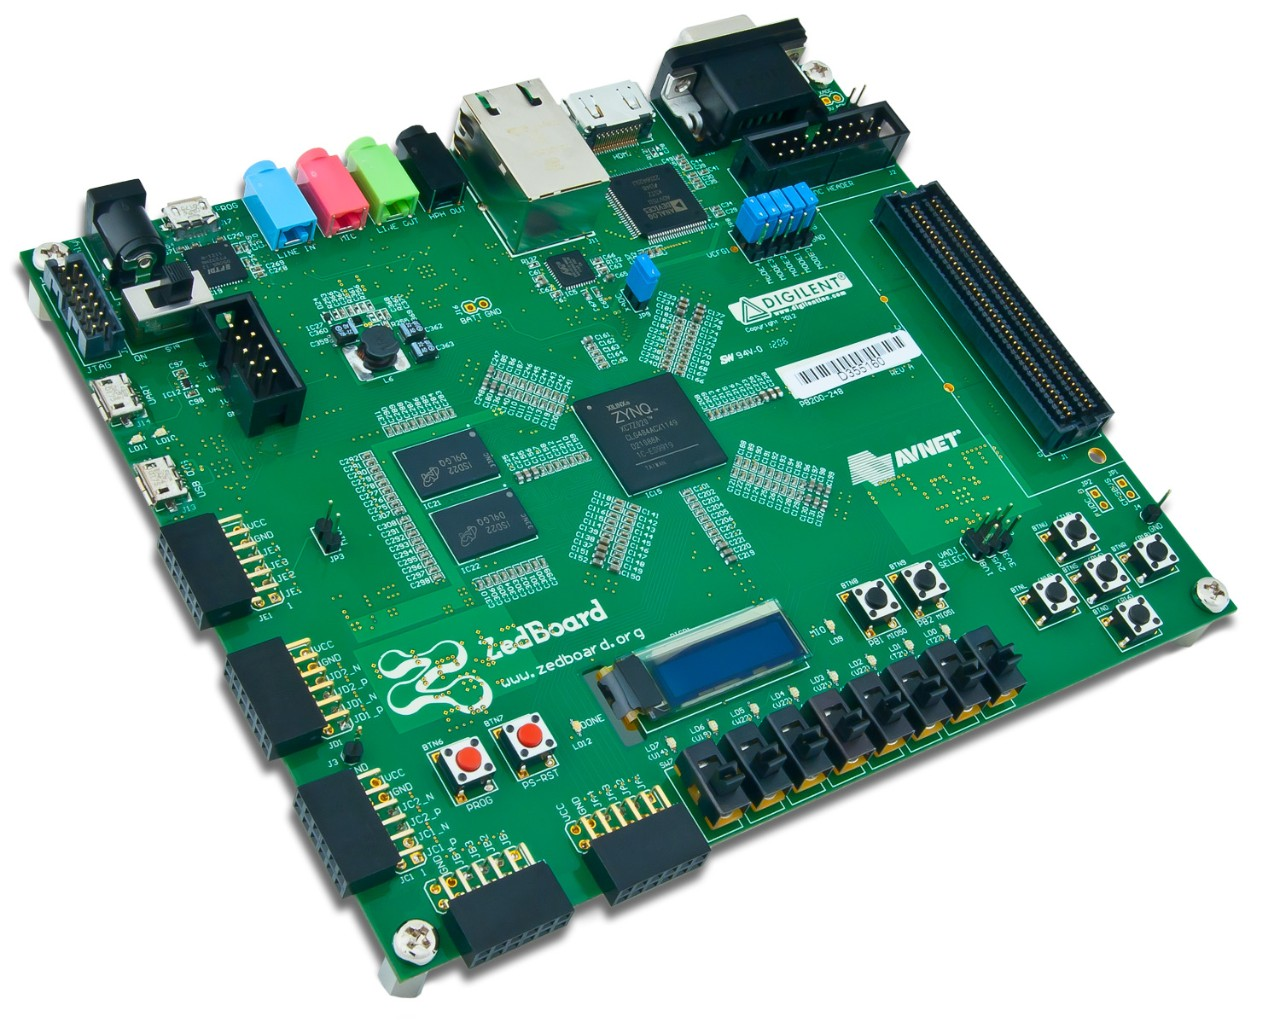
\includegraphics[width=\textwidth]{./img/zedboard.jpg}
\caption{Zeboard}
\end{subfigure}
\begin{subfigure}[b]{0.3\textwidth}
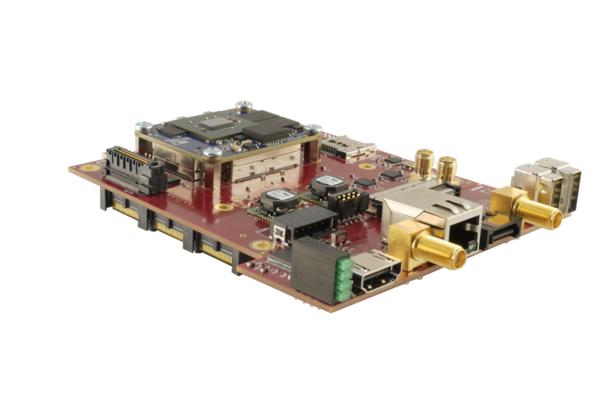
\includegraphics[width=\textwidth]{./img/emc2dp.jpg}
\caption{EMC2DP}
\end{subfigure}
\caption{}
\label{fig:development_boards}
\end{figure}

\section{Hardware}
The Zynq-7000 SoC has a Processing System (PS) consisting of a hardwired application processing unit, memory controller, and peripheral devices. The main processing unit is a dual-core Cortex-A9 ARM processor. Connected to the PS region is a Programmable Logic (PL) region. The PL is based on Xilinx’s 7-series FPGA technology.\\

Both the PS and PL regions have support for ARM TrustZone~\cite{website:ARM}.\\

\section{Operative systems}
The Alten MCS uses two Operative Systems (OS) to create temporal and spatial separation between safety-critical and non-critical applications using TrustZone. In its current setup the Real-Time Operative System (RTOS) FMP by TOPPERS~\cite{website:fmp} is used for safety-critical applications. This RTOS follows the uITRON4.0 specification~\cite{uitron}, which is a widely used RTOS specification for Japanese embedded systems. For non-critical applications, the General Purpose Operative System (GPOS) Linux kernel 4.4 is used. Instead of Linux another instance of FMP could be used for non-critical applications.\\

Tasks in FMP are statically allocated to a processor core, defined in a .cfg file. Linux divides its workload across all available processor cores in SMP (Symmetric Multi-Processor) mode.

\section{Hypervisor}
%TODO: timings for switching
%The hypervisor SafeG is used to alternate between the safety-critical (S\_OS) and non-critical (NS\_OS) OS. It switches processor state via a hardware switch. See figure~\ref{fig:modeswitch}. The switching takes ~2 $\mu s$.

A hypervisor (also known as a Virtual Machine Monitor (VMM)) is used to alternate between the safety-critical (S\_OS) and non-critical (NS\_OS) OS. The hypervisor used is SafeG \cite{website:safeg}, also developed by TOPPERS. It switches processor state via a hardware switch. See figure~\ref{fig:modeswitch}. The switching takes roughly 2~$\mu s$~\cite{safegswitch}.

\begin{figure}[H]
\centering
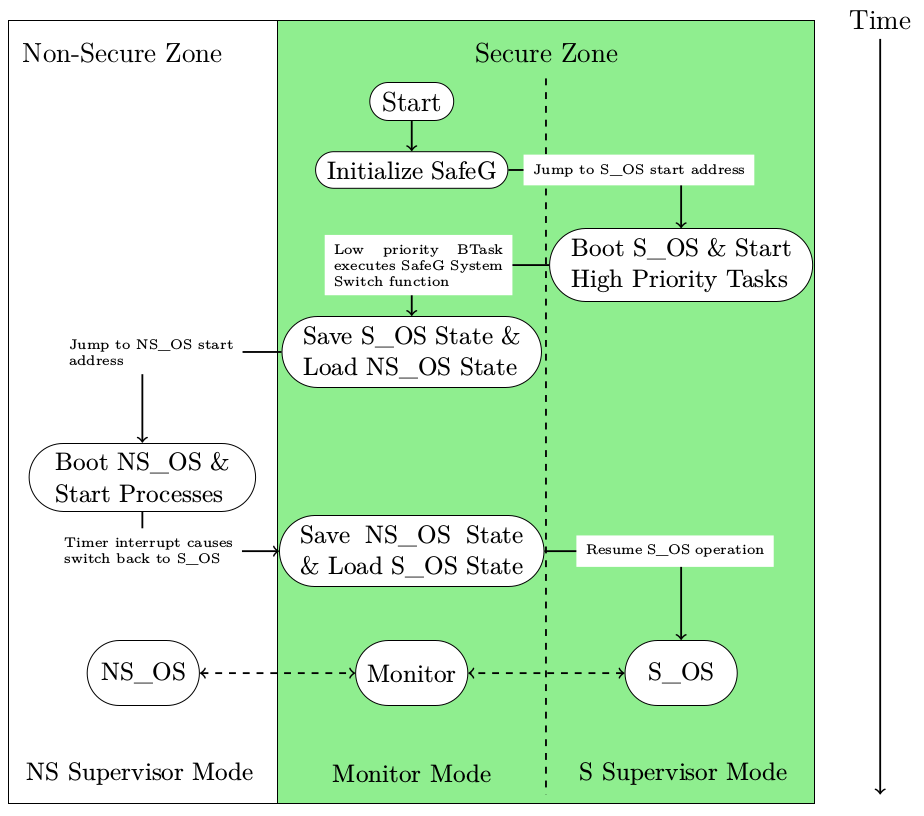
\includegraphics[width=\textwidth]{./img/literature_modeswitch.png}
%Flowchart of how the physical CPU switches between the virtual CPUs
\caption{Flowchart of the boot sequence of the CPU. \cite{zaki2016}}\label{fig:modeswitch}
\end{figure}

%TODO: gör okefft
For the hypervisor, the GPOS is regarded as another task with lowest priority. \\

The time it takes the hypervisor to switch processor state bounds the maximum frequency a task can have while the processor still manages to maintain its switching capabilities. The maximum frequency, $f_{max}$, can be calculated as

$$f_{max} = \lim_{e_s, e_{ns} \to 0} \frac{1}{e_s+e_{ns}+2e_{switch}} = 250\textrm{ kHz}$$

where $e_s$ is the execution time of the tasks on the S\_OS, $e_{ns}$ is the execution time of the tasks on the NS\_OS and $e_{switch}$ is the time required for the mode-switch.\\

A basic overview of the hardware and the software of the system can be seen in Figure~\ref{fig:system_overview}.

\begin{figure}[H]
\centering
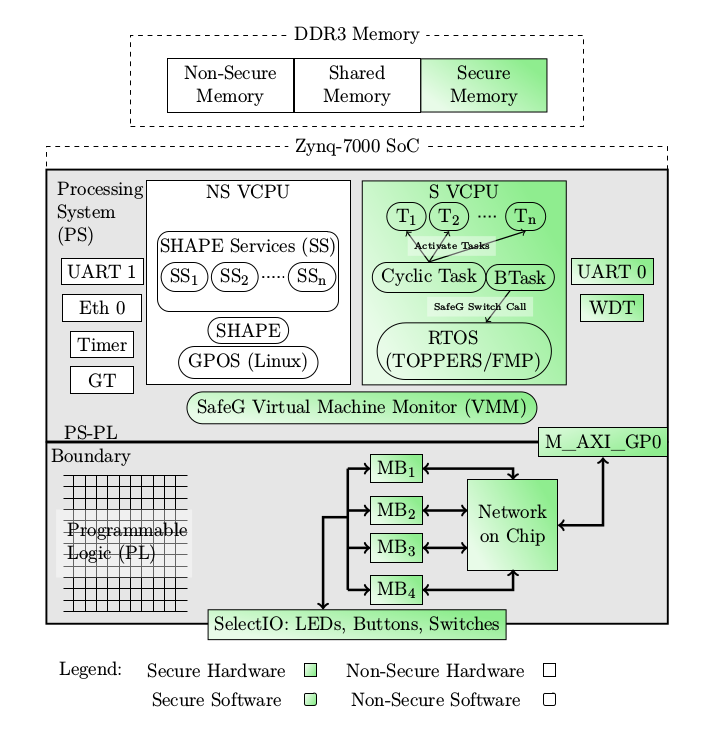
\includegraphics[width=\textwidth]{./img/literature_overview.png}
\caption{Overview of the MCS in place.\cite{zaki2016}}\label{fig:system_overview}
\end{figure}

\section{Build procedure}
The MCS is built from many different components. Hardware design,  applications, virtualization layer, operative systems, boot loaders etc. This section will describe the build procedure.\\ %TODO: Expand
%The virtualization layer (SafeG) and the Secure OS (RTOS) remain the same, the software that runs in the normal region can be either RTOS, GPOS, or a bare metal application. Furthermore, other configurations, such as RTOS or GPOS only mode, do not include the VMM.

Xilinx's software Vivado HLS~\cite{website:vivado} is used to design the FPGA of the Zynq-7000. In Vivado the different IPs, their interconnect and the Processing System is configured. This results in a bitstream file that is used in Xilinx SDK to generate a Board Support Package (BSP) and the First Stage Boot Loader (FSBL). The BSP contains libraries for functions and variables necessary for the IPs on the FPGA, and the FSBL configures the FPGA correctly. The FSBL is included in the boot file (BOOT.bin) generated in Xilinx SDK. The boot file also contains the Second Stage Boot Loader (SSBL), u-boot. U-boot is a program that can load executables and other system files from a remote server into the DDR3 memory. This is used to load relevant files for the OS into the Zynq, which brings us to the software part of the build procedure. The software is divided into three parts: RTOS, GPOS and monitor. The SafeG monitor is built and compiled using GCC (Gnu Compiler Collection), resulting in monitor.bin. The RTOS FMP is built and compiled from a .cfg file where tasks and handlers are created, a .c file where tasks and handlers are defined and a .h file containing declarations. This results in fmp.bin. For the non-secure side either Linux or another instance of FMP could be used. The process for FMP is the same as with the secure side. For Linux on the non-secure side, the Linux kernel needs to be modified to support SafeG. This results in the files zImage, devicetree.dtb. All of these files are created and stored on a server and are then loaded into the Zynq-7000 using u-boot.\\
%, only using the declaration #ifdef TOPPERS_SAFEG_NONSECURE

%Xilinx's software Vivado~\cite{website:vivado} is used to synthesize the hardware design (vhdl or verilog code) into a bitstream file (.bit) in order to configure the PL region of the Zynq. Vivado also produces a set of files that represent the designed hardware platform, which are used for software development. Xilinx SDK tool is used to create the Board Support Package (BSP) and the First Stage Boot Loader (FSBL) that correspond to the designed system. In general, after the FSBL initialization process completes, and depending on boot sequence, the CPU can do any of the following actions: configure the FPGA, initiate the Second Stage Boot Loader SSBL, or jumps to the first address of the main program. The SDK tool is also used to generate a boot file (BOOT.bin), which must at least contain the FSBL (fsbl.elf). In the implemented system, the BOOT.bin file also includes the bitstream file (system.bit) and the SSBL (uboot.elf * ). Once the system is initialized and the PL is configured, the system starts executing the u-boot instructions present in the BOOT.bin. U-boot is a full system on its own, and has many useful features. In particular, u-boot can be used to load executables and other system files from a remote server into the DDR3 memory using protocols such as Trivial File Transfer Protocol (TFTP), see Figure~\ref{fig:system_build}.\\

Figure \ref{fig:system_build} provides a summary of the different dependencies for the system and the required flow for building the system.

%TODO: NY BILD

\begin{figure}[H]
\centering
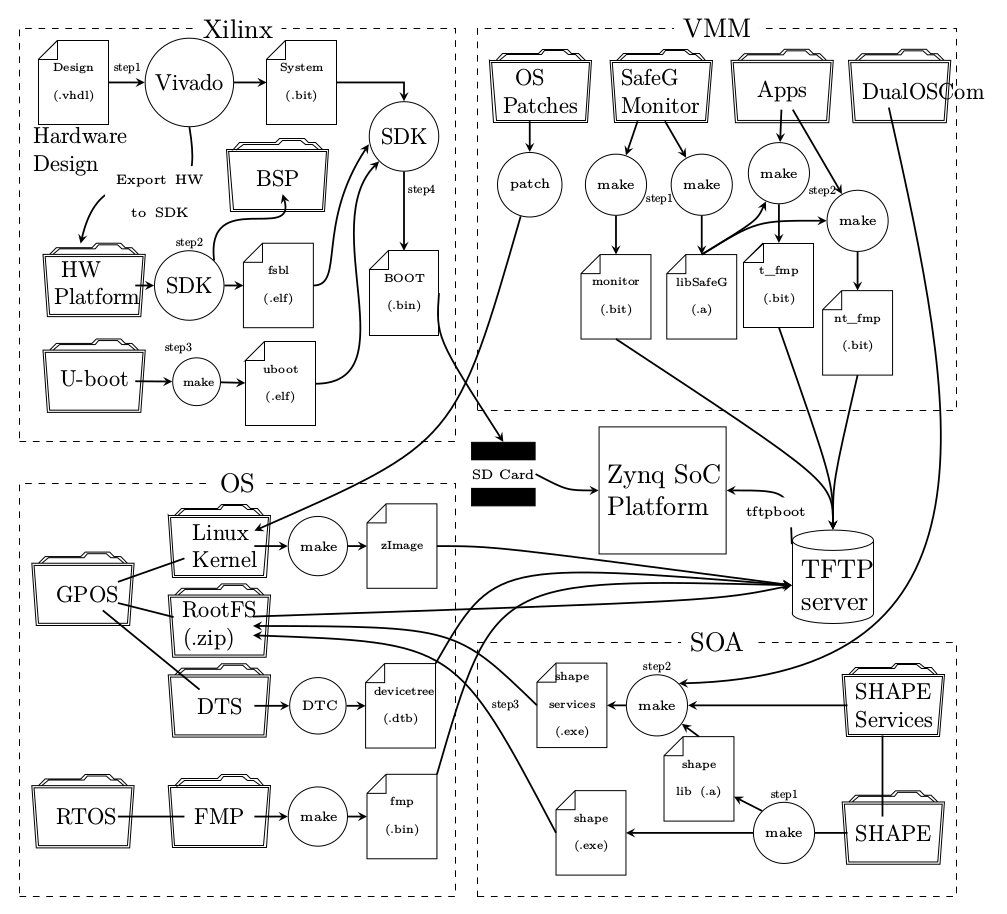
\includegraphics[width=\textwidth]{./img/literature_build.png}
\caption{System build procedure.\cite{zaki2016}}\label{fig:system_build}
\end{figure}

%For more information about the build and the system, see the report by Zaki~\cite{zaki2016}.

This build procedure setup provides for easy modifications to a small part of the system without having to rebuild other parts, and the board to which the code should be loaded into only needs to be connected to a network socket and a laptop.
%TODO: rephrase